\section{Background\label{introduction:background}}

\subsection{Breast Cancer Overview\label{sec:introduction:breastcanceroverview}}
Breast cancer is a type of cancer that starts in one or both breasts.

\subsubsection{Statistics\label{sec:introduction:breastcancer:statistics}}
Breast cancer accounts for about 30\% of all new cancer cases in U.S. women each year~\cite{RefWorks:RefID:150-2025breast}. The average risk of a woman in the U.S. developing breast cancer sometime in her life is about 1 in 8 (about 13\%)~\cite{RefWorks:RefID:36-american2021breast}. Breast cancer is also the second leading cause of cancer death in women behind lung cancer~\cite{RefWorks:RefID:36-american2021breast}.

\subsubsection{Development and Spread\label{sec:introduction:breastcancer:developmentandspread}}
Breast cancer can start in different parts of the breast, such as the ducts, lobules, or the tissue in between. The cancer can spread when cancer cells are carried to other parts of the body through blood or the lymphatic system. The lymphatic system is a network of small bean-sized glands called lymph nodes, ducts, and vessels that carry clear lymph fluid throughout the body. This clear lymph fluid contains immune system cells to fight infection as well as waste and tissue by-products. This system carries lymph fluid away from the breast; cancer cells can enter the lymph vessels, grow inside lymph nodes, and spread to other parts of the body~\cite{RefWorks:RefID:36-american2021breast}.

The most common areas where lymph vessels of the breast drain into are the underarm (axillary), inside the chest near the breastbone (internal mammary), and around the collar bone (supraclavicular and infraclavicular). Once cancer cells have spread to  the lymph nodes, there is a higher chance of metastases, or spreading, to other parts of the body which is called metastatic breast cancer~\cite{RefWorks:RefID:36-american2021breast}.

The method of cancer cells metastasizing through the lymphatic system is illustrated below in Figure~\ref{fig:introduction:process_of_metastatic_breast_cancer}.

\begin{figure}[h!]
        \centering
        \fbox{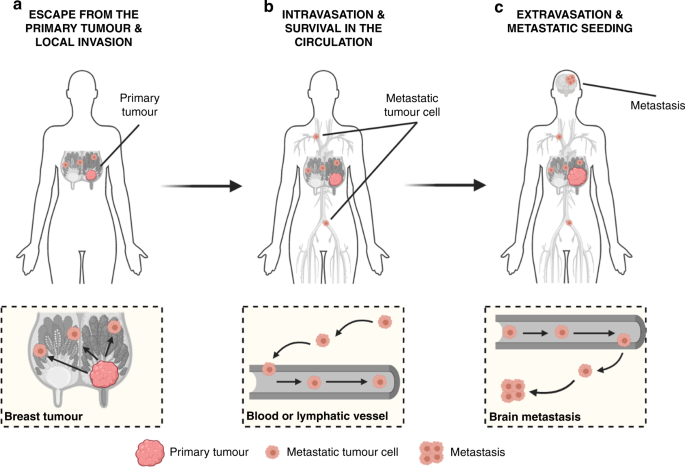
\includegraphics[width=0.8\textwidth]{../figs/introduction/process_of_metastatic_breast_cancer.png}}
        \caption{Process of Metastatic Breast Cancer \cite{RefWorks:RefID:364-riggio2020lingering}.}
        \label{fig:introduction:process_of_metastatic_breast_cancer}
\end{figure}

\subsection{Treatment of Breast Cancer\label{sec:introduction:treatmentofbreastcancer}}

\subsubsection{Stages of Breast Cancer\label{sec:introduction:breastcancer:stagesofbreastcancer}}
% Early vs late stage

\subsubsection{Current Treatment Options\label{sec:introduction:breastcancer:currenttreatmentoptions}}
% Lumpectomy vs mastectomy

\subsection{Motivation\label{sec:introduction:motivation}}
This is a subsection of the background in the introduction!
